\documentclass{edm_template}

%\usepackage{amsthm,amsmath,amsfonts}
\usepackage{bm}
\usepackage{comment}
\usepackage{multirow}

\newcommand{\tauhat}{\hat{d}^{np}}
\newcommand{\shrink}{\hat{d}^{pp}}
\newcommand{\EE}{\mathbb{E}}
\newcommand{\tshrink}{T^{pp}}

\newtheorem{prop}{Proposition}


\begin{document}

\title{Bayesian Partial Pooling to Improve Inference Across A/B Tests in EDM}

\numberofauthors{3} 
\author{
% 1st. author
\alignauthor Adam C Sales\\
       \affaddr{University of Texas at Austin}\\
       \affaddr{536C George I. S\'{a}nchez Building}\\
       \affaddr{Austin, TX 78705}\\
       \email{asales@utexas.edu}
% 3rd. author
\alignauthor Thanaporn Patikorn\\
\affaddr{Worcester Polytechnic Institute}
       \affaddr{100 Institute Rd}\\
       \affaddr{Worcester, MA 01609}\\
       \email{tpatikorn@wpi.edu}
\and  % use '\and' if you need 'another row' of author names
% 4th. author
\alignauthor Neil T. Heffernan\\
\affaddr{Worcester Polytechnic Institute}
       \affaddr{100 Institute Rd}\\
       \affaddr{Worcester, MA 01609}\\
       \email{nth@wpi.edu}
}

\maketitle
\begin{abstract}
This paper will explain how analyzing experiments as a group can improve estimation and inference of causal effects--even when the experiments are testing unrelated treatments. The method, composed of ideas from meta-analysis, shrinkage estimators, and Bayesian hierarchical modeling, is particularly relevant in studies of educational technology. Analyzing experiments as a group--"partially pooling" their respective datasets--increases overall accuracy and avoids issues of multiple comparisons, while incurring small bias. The paper will explain how the method works, demonstrate it on a set of randomized experiments run within the ASSISTments platform, and illustrate its properties in a simulation study.
% * <neiltheffernaniii@gmail.com> 2018-03-07T16:39:34.243Z:
% 
% What does desing based methods mean? Is that a techincal term?
% 
% ^.
\end{abstract}

\section{Introduction}
Educational technology can be a boon to education and cognitive science research in general.
One of the most prominent ways this is so is the ease of conducting randomized experiments, or A/B tests.
For instance, the ASSISTments TestBed \cite{testbed} is an online platform that allows researchers to conduct randomized experiments within the ASSISTments intelligent tutoring system, and makes the data publicly available. 
Clearly, the ability to conduct many experiments allows education researchers to ask many questions and test many hypotheses independently.
Perhaps more surprisingly, the various experiments can help \emph{each other}.
Effect estimates that partially pool data across experiments---even those that are testing very different interventions---are often more precise and accurate, and less error-prone, than estimates based on the experiments individually. 

This paper will illustrate a Bayesian approach to analyzing several experiments simultaneously.
The method combines ideas from \cite{jamesStein} and \cite{efronMorris} on improvements in precision due to pooling, from \cite{rubin} on Bayesian partial pooling to examine treatment effect heterogeneity, and \cite{gelmanMultiple} on partial pooling to avoid problems arising from multiple comparisons. 
The paper's main contributions will be to introduce these ideas to an EDM audience---where they are particularly applicable---and to illustrate their potential.

After describing and explaining the method (Sections \ref{sec:shrinkage}--\ref{sec:multipleComparisons}), we will illustrate it in an analysis of a dataset comprised of 22 parallel experiments run inside ASSISTments \cite{data} (Section \ref{sec:experiments}) and in a simulation study (Section \ref{sec:simulation}). We will show that partially pooling data from across experiments increases precision while lowering type-I error rates, decreases the width of confidence intervals while improving their coverage, addresses issues of multiple comparisons, and substantially reduces the incidence of drawing incorrect conclusions from experimental data. 

\section{Shrinkage, Partial Pooling, and Regression to the Mean}\label{sec:shrinkage}
Unbiased estimates $\tauhat$ of effect sizes $d$ from randomized A/B tests are noisy---a different estimate would have resulted had the treatment been randomized differently.
The standard error of a particular effect size estimate, $\sigma_i=SD(\tauhat_i|d_i)$, depends on a number of factors, most principally the sample size $n_i$, but in practice it is never zero.
Similarly, among a group of $K$ experiments, the true effect sizes $d_i$, $i=1,...,K$, (presumably) vary as well---$var(d)=\tau$, say. 
Considered together, the variance of a group of effect size estimates is the sum of both components: the variance of the true effects plus the average of the (squared) standard errors of the individual estimates:
\begin{equation*}
var(\tauhat)=\tau^2+\EE[\bm{\sigma^2}]
\end{equation*}
In other words, the distribution of effect size \emph{estimates} is wider than the distribution of true effect sizes.
It follows that the largest effect size estimates $\tauhat$ more likely than not \emph{over}estimate their respective true effects $d$, and that the smallest effect size estimates probably \emph{under}estimate their true effects.
This is an example of regression to the mean \cite{galton}.

The implication for estimating effects can be startling.
When A/B tests are analyzed independently, the best estimate for the true effect size $d_i$ in experiment $i$ is $\tauhat_i$.
However, when the $K$ experiments are considered as a group, $\tauhat$ is inadmissible.
A better estimate, $\shrink$, corrects for the fact that the extreme estimates are probably too extreme, and shrinks them toward the overall mean effect size $\mu$ \cite{efron1977stein}:
\begin{equation}\label{eq:shrinkage}
\shrink_i=\mu+c_i\left(\tauhat_i-\mu\right)
\end{equation}
where $c_i$ is a ``shrinkage coefficient'' between 0 and 1. 
When $c_i=1$, $\shrink_i=\tauhat_i$; when $c_i=0$, $\shrink_i=\mu$.

Another term for this procedure is ``partial pooling'' \cite{gelmanHill}.
The overall mean treatment effect, $\mu$, can be estimated by completely pooling the data across all $K$ experiments.
In contrast, individualized estimates $\tauhat$ result if data from different A/B tests are not pooled at all---$\tauhat$ is a ``no pooling'' estimate.
The optimal estimate $\shrink$ combines the the no-pooling estimate $\tauhat$ with a complete-pooling estimate of $\mu$---hence, partial pooling. 

In general, the size of the shrinkage coefficient $c_i$, which regulates the extent of the partial pooling, depends both on the standard deviation of the true effects, $\tau$, and $\sigma_i$, the standard error of $\tauhat_i$.
When $\tau$ is large, the experiments differ widely from each other, so the overall mean effect $\mu$ tells us little about the individual effects $d$.
When $\sigma_i$ is large, then $\tauhat_i$ is quite noisy, and tells us little about $d_i$.
The shrinkage coefficient $c_i$ balances these two factors. 

For instance, Rubin \cite{rubin} models each $\tauhat_i$ as normal, with mean $d_i$ (since it is unbiased) and standard error $\sigma_i$:
\begin{equation}\label{eq:estimateModel}
\tauhat_i\sim\mathcal{N}\left(d_i,\sigma_i\right)
\end{equation}
This would be approximately the case if estimators $\tauhat$ were difference-in-means or regression estimators from sufficiently large experiments.
Then, he models the effects themselves as drawn from a normal distribution:
\begin{equation}\label{eq:effectModel}
d_i\sim\mathcal{N}(\mu,\tau).
\end{equation}
Under model (\ref{eq:estimateModel})--(\ref{eq:effectModel}), 
\begin{equation}\label{eq:shrinkageCoef}
c_i=\frac{\tau^2}{\tau^2+\sigma_i^2}.
\end{equation}
When $\tau$ is large (so the true effects are very different from each other) and $\sigma_i$ is small (so $\tauhat_i$ is very precise), $c_i$ is close to one---the partial pooling estimator $\shrink_i \approx \tauhat_i$---data are barely pooled across experiments at all. 
Conversely, when $\sigma_i$ is large (so $\tauhat_i$ is noisy) and $\tau$ is small (so the true effects are similar to each other), then $c_i$ is close to zero, and $\shrink\approx \mu$, the overall mean effect size, completely pooling data across experiments. 
In general $c_i$ is in between zero and one, and the estimator $\shrink$ partially pools information between the individual effect estimate $\tauhat_i$ and the overall mean $\mu$.
The mean of the true effects $\mu$ and their variance $\tau$ are, of course, unknown, but they may be estimated from the data. 

Truman Kelley \cite{kelley} first derived the partial pooling estimator $\shrink$ in 1927, in the context of educational testing, to estimate a student's ``true'' test score from her estimated score.
Charles Stein \cite{stein} showed that Kelley's principle applied much more broadly.
In any collection of $K\ge 3$ estimation problems, the optimal estimates must involve shrinkage.
What's so shocking about this result is that the estimation problems do not need to be related in any way. 
As \cite{stigler} put it (pp. 147--148), 
\begin{quote}
 When this phenomenon is first encountered it can
 seem preposterous---how can (to use a variant of an
 early illustration) information about the price of apples in Washington and about the price of oranges in
 Florida be used to improve an estimate of the price of
 French wine, when it is assumed that they are unrelated?
\end{quote} 
Nevertheless, as $\cite{stigler}$ shows and we have seen, the result is a consequence of regression to the mean. 

Partial pooling is inherently a compromise: unlike $\tauhat_i$, $\shrink_i$ is biased---it is shrunk towards the overall mean $\mu$.
To compensate for the bias, $\shrink_i$ is less noisy than $\tauhat_i$; its standard error is $\sqrt{c_i} \sigma_i$.
Since $c_i<1$, this is always less than $\tauhat_i$'s standard error $\sigma_i$. 
Overall, \cite{stein} shows the mean squared error (MSE) of the estimates $\shrink$, considered as a group, will be less than the MSE of the individual unbiased estimates $\tauhat$.

When analyzing a set of A/B tests run inside intelligent tutors, estimates of the effects based on partial pooling will be more accurate, on average, than estimates that consider each test individually.

\section{Multiple Comparisons}\label{sec:multipleComparisons}
The standard practice when analyzing A/B tests is to report effect estimates alongside statistical significance, typically at the $\alpha=0.05$ level.
When reporting multiple results simultaneously, this can lead to problems of multiple comparisons.
For each test individually, if the null hypothesis is true---i.e. there is no treatment effect---the probability of a statistically significant result, in this case a ``type-I error,'' is $\le 0.05$ (assuming proper statistical methods).
However, the probability of at least one significant result from multiple experiments testing null effects is typically greater than 0.05. 
For instance, in 20 independent experiments with no true effects present, the probability of at least one spuriously significant result is roughly 0.64. 

Fortunately, this appears not to be the case when estimating effects via partial pooling.
The argument, presented in \cite{gelmanMultiple}, is as follows.
Significance in experiment $i$ is typically assessed via a test statistic of the form $T_i=\tauhat_i/\hat{\sigma}_i$.
$T$ statistics that are much larger in magnitude than expected under the null hypothesis are statistically significant. 
Spurious significance is the result of (spuriously, randomly) large effect estimates $\tauhat$---the more A/B tests run, the more likely a surprisingly large $\tauhat$ becomes, even when no true effect is present. 

However, when all true effects are zero, $\mu=0$.
Therefore the partial-pooling $T$ statistic is 
\begin{equation*}
\tshrink_i=\frac{\shrink_i}{\sqrt{c_i}\sigma_i}=\frac{c_i\tauhat_i}{\sqrt{c_i}\sigma_i}=\sqrt{c_i}T_i<T_i
\end{equation*}
Since $\shrink$ is shrunk towards the mean of the treatment effects (in this case, 0), spuriously large values of $\shrink$, and hence $\tshrink$, become less likely.
(When all treatment effects are zero, $\tau=0$ as well, implying that $c_i=0$. Here the fact that $\mu$, $\tau$, and $\sigma_i$ must all be estimated from the data becomes important---the estimate of $\tau$ will never be exactly zero, but might be quite low.)

\subsection{Type-S and Type-M Errors}
Actually, the argument in \cite{gelmanMultiple} is not exactly as above. Statistical significance testing seeks to minimize type-I errors, in which researchers mistakenly conclude that an effect is non-zero.
The authors of \cite{gelmanMultiple} contend that, in reality, treatment effects are never exactly zero, though they may be quite small. 
Instead, they argue for focusing on two other types of errors.
A ``type-S'' error is an error in the sign of the effect, when a researcher concludes that an average effect is positive, when it is, in fact, negative, or vice versa.
A ``type-M'' error is an error in magnitude, when a research concludes than an effect is large, when in reality it is small, or vice-versa.

It turns out that classical significance testing when power is low can induce both type-S and type-M errors. 
For instance, if a true effect $d$ is positive, say $d=0.02$, and it is estimated by an unbiased estimator $\tauhat$ which is normally distributed with mean $0.02$ and standard error $\sigma=0.1$. 
Then the power---the probability of a statistically significant result---is 0.055.
However, about 28\% of these significant results will be of the wrong sign---that is, 28\% of the time a researcher detects a significant effect, the direction of the effect will be wrong, a type-S error.
Further, in order to achieve statistical significance, the effect must be over-estimated.
The smallest possible significant effect has a magnitude of 1.96 times the estimated standard error.
In this case, if the standard error is estimated accurately, a significant estimate must be almost 10 times the true effect, a type-M error. 
When multiple A/B test results are reported together, the probability of significant effect estimates increases, and so do the probabilities of type-S and type-M errors. 

Fortunately, \cite{gelmanMultiple} argues that partial pooling alleviates the multiple comparisons problem with regard to type-S and type-M errors, in just the same way it reduces the rate of type-I errors. 

\section{Analyzing 22 Experiments}\label{sec:experiments}
How does partial pooling work in practice, in an authentic EDM setting?

%  Ostrow, K.S., Heffernan, N.T., & Williams, J.J. (2017). Tomorrow’s EdTech Today: Establishing a Learning Platform as a Collaborative Research Tool for Sound Science. Teachers College Record, Volume 119 Number 3, 2017, p. 1-36.

The ASSISTments TestBed \cite{testbed} allows education researchers to propose and conduct minimally-invasive A/B tests within the ASSISTments intelligent tutor. The TestBed infrastructure automatically publishes anonymized data from these experiments.
Conveniently, \cite{data} combined 22 of these datasets into one publicly available file.
All 22 experiments were skill builders, which are problem sets designed to teach, or bolster, a specific topic or skill.
Inside a skill builder, students are required to solve problems associated to that skill until mastery is achieved, typically defined as answering three questions in a row. 

The dataset includes a number of student features and two dependent measures. In this paper, We will focus only on one dependent measure \texttt{complete}.
\texttt{complete} is a binary variable indicating completion of the skill builder, taking value 1 if the student achieved mastery or 0 if the student either stopped working before achieving mastery or exhausted all of the skill builder's problems without achieving mastery. 

To estimate treatment effects conventionally, without pooling across experiments, we fit a separate logistic regression to each of the 22 experiments, regressing \texttt{complete} on an indicator for treatment condition.
The estimated treatment effect was the coefficient on the condition indicator, equal to the log odds ratio of completion for the treatment vs the control condition.

To estimate effects using, partial pooling, we fit a Bayesian multilevel logistic regression using the Stan Markov Chain Monte Carlo sampler, called from \texttt{R} \cite{rcite} via the \texttt{rstanarm} package \cite{rstanarm}. 
The model was 
\begin{equation*}
Pr(complete=1)=invLogit\left(\alpha_{expr}+\beta_{expr}Z\right)
\end{equation*}
where $\alpha_{expr}$ is a random intercept for each experiment, modeled as normal, $\beta_{expr}$ is a separate treatment effect estimate (log odds ratio) for each experiment, also estimated as normal, and $Z$ is an indicator for the treatment condition.

\begin{figure}
\centering
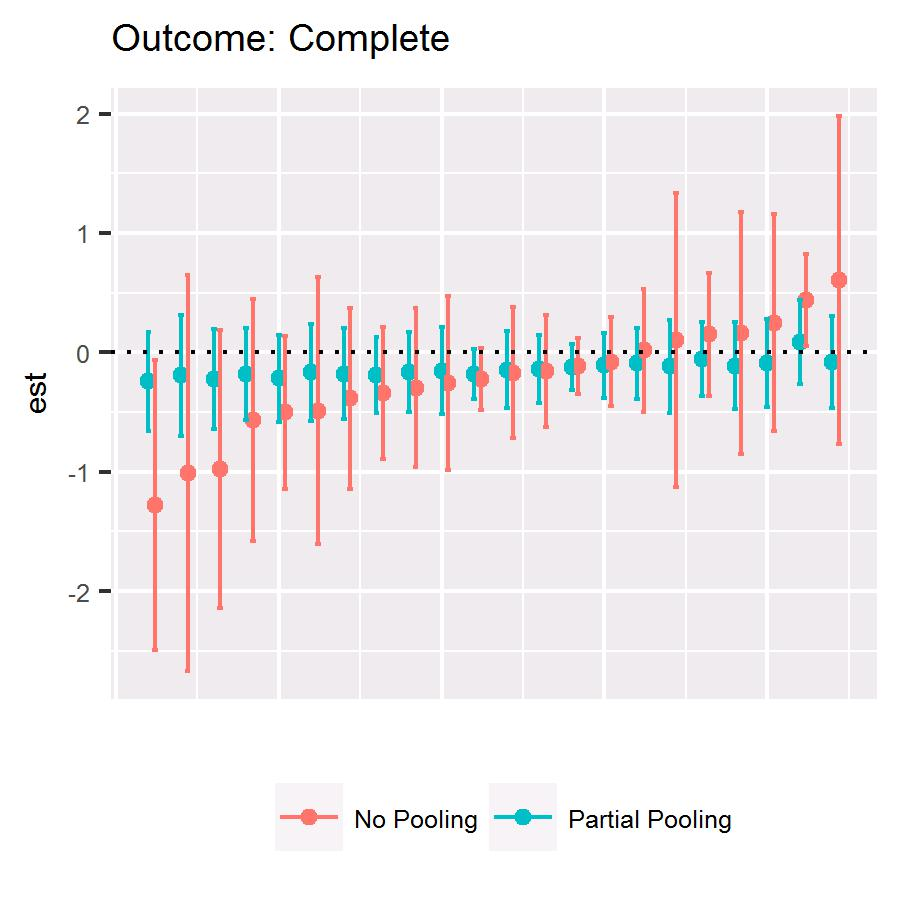
\includegraphics[width=0.45\textwidth]{completeEst1.jpg}
\caption{Partial-pooling an no-pooling treatment estimates and approximate 95\% confidence intervals for the 22 experiments, arranged horizontally by the no-pooling treatment effect. The outcome was \texttt{complete}, and the treatment effects are log-odds ratios.}
\label{fig:estimates}
\end{figure}

Figure \ref{fig:estimates} plots estimated treatment effects and approximate 95\% confidence intervals ($\pm 2SE$) for the 22 experiments, using both the conventional no-pooling estimator and the partially-pooling estimator. 
The partial pooling shrunk the estimates quite a bit: while the no-pooling estimates ranged from approximately -1.3 to 0.6, the partial pooling estimates were all close to zero, ranging from -0.2 to  0.1. 
The estimated standard errors were also much smaller for the partially pooled estimators.
The average standard error for the no-pooling estimates was 0.39, whereas the average standard error for the partial-pooling estimates was less than half that, 0.17.
Finally, though two of the no-pooling estimates were statistically significant, with confidence intervals excluding zero, none of the partial-pooling estimates was. 


\begin{figure}
\centering
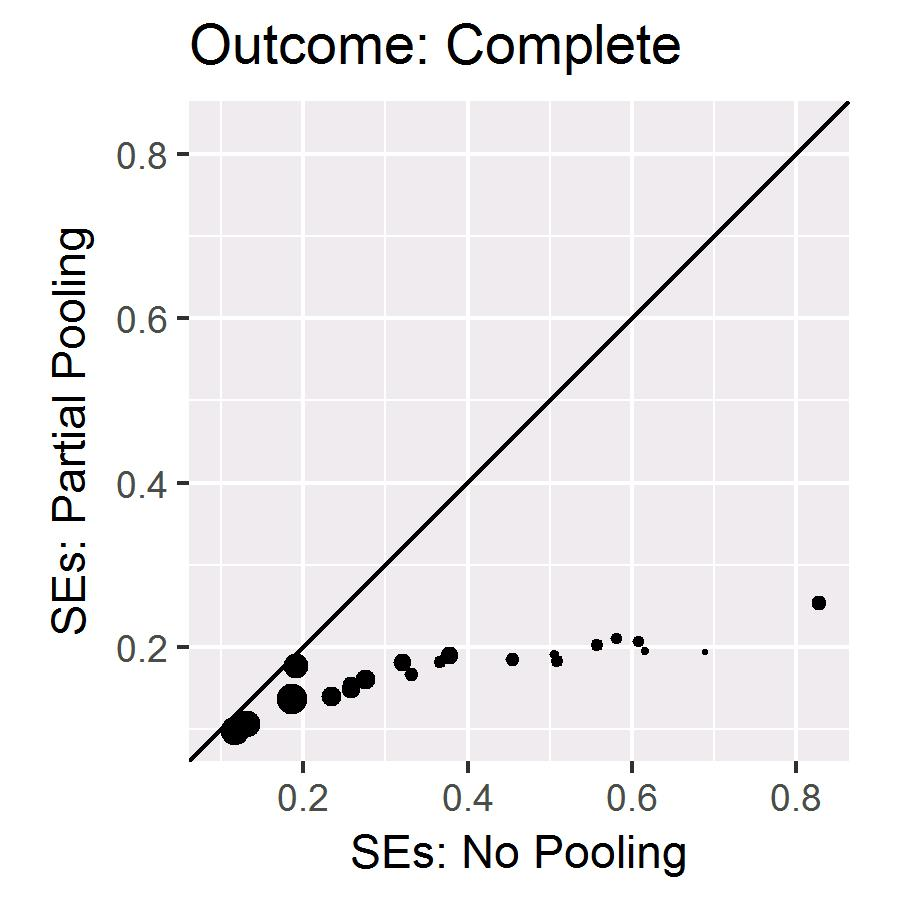
\includegraphics[width=0.45\textwidth]{completeSE1.jpg}
\caption{Partial-pooling vs no-pooling standard errors, with point size proportional to sample size in the experiment.}
\label{fig:ses}
\end{figure}

Figure \ref{fig:ses} plots the estimated standard errors from the two sets of estimates. 
The sizes of the points in the plot are proportional to experimental sample sizes.
The partial-pooling standard errors are all smaller than those from the no-pooling estimates.
However, the differences are not uniform. 
Experiments with large sample sizes and low no-pooling standard errors had partial-pooling standard errors that were only slightly smaller. 
As the sample sizes shrunk, both sets of standard errors grew.
However, the no-pooling standard errors grew much faster. The largest difference in standard errors between the two methods was for studies with the smallest samples and the largest no-pooling standard errors. 


\section{A Simulation Study}\label{sec:simulation}
Partial pooling worked as advertised when applied to the ASSISTments dataset, shrinking estimates towards zero and reducing standard errors, sometimes drastically---but did it get the right answers? 

We ran a simulation study to investigate the performance of the partial-pooling estimator when the right answer is known.

\subsection{Data Generating and Analysis Models}
We simulated batches of $K=20$ experiments each.
Within a batch, sample sizes $n$ varied from 20 to 115.
Treatment $Z$ was randomized to half of the subjects in each experiment.
For each batch, outcomes $Y$ were generated as 
\begin{equation}\label{eq:dgm}
Y_i\sim \mathcal{N}(\alpha_{expr[i]}+\beta_{expr[i]}Z_i,1)
\end{equation}
with random intercepts $\alpha_{expr}\sim\mathcal{N}(0,1)$ and treatment effects $\beta_{expr}\sim\mathcal{N}(0,\tau)$, both varying at the experiment level.
The between-experiment standard deviation of treatment effects $\tau$ varied between runs. 
It took the values of $\tau=0$, corresponding to $\beta_{expr}\equiv 0$ across all experiments, and $\tau=\{0.1,0.2,0.5,1.0\}$.
When $\tau$ was positive but low, there was a treatment effect in every experiment, but nearly all effects were very small.
Larger values of $\tau$ corresponded to more variance in the treatment effects, including some that were substantial. 
For comparison purposes, the pooled standard deviation of $Y$ within each study was 1; across studies it was the square root of the sum of the variance of $\alpha_{expr}$ and the residual variance, or $\sqrt{2}$.

The 20 experiments in each batch were analyzed both separately, with no-pooling estimators, and jointly, with a partial-pooling estimator. 
The no-pooling estimator was the simple difference in means, $\tauhat=\bar{Y}_{Z=1}-\bar{Y}_{Z=0}$, with the conventional standard error estimate.
We used \texttt{rstanarm} to compute the partial pooling estimator, fitting a multilevel linear regression model equivalent to the data generating model (\ref{eq:dgm}) but with all means and variances estimated from the data.

For each value of $\tau$ we ran 500 iterations of 20 experiments each, producing 10,000 experimental datasets.

\subsection{Simulation Results}
\begin{table*}
\centering
\begin{tabular}{rrlllll}
&&\multicolumn{5}{c}{$\tau$}\\
&&0&0.1&0.2&0.5&1\\
\hline
\multirow{2}{*}{ Standard Error }& Partial Pooling & 0.13&0.14&0.17&0.23&0.25 \\ 
& No Pooling & 0.26&0.27&0.26&0.27&0.26 \\ 
\hline\multirow{2}{*}{ $|$Bias$|$ }& Partial Pooling & 0.00&-0.05&-0.08&-0.08&-0.05 \\ 
& No Pooling & 0.00&-0.00&0.00&0.00&0.00 \\ 
\hline\multirow{2}{*}{ RMSE }& Partial Pooling & 0.09&0.12&0.17&0.24&0.26 \\ 
& No Pooling & 0.28&0.27&0.27&0.28&0.27 \\ 
\hline\multirow{2}{*}{ 95\% CI Coverage }& Partial Pooling & 1.00&0.98&0.95&0.95&0.95 \\ 
& No Pooling & 0.95&0.95&0.95&0.95&0.95 \\ 
\hline
\end{tabular}
\caption{Average standard error, bias magnitude, root mean squared error (RMSE), and empirical coverage of 95\% confidence intervals for partial pooling and no pooling estimates for different values of $\tau$, the standard deviation of treatment effects, in the simulation study.}
\label{tab:simRes1}
\end{table*}

\begin{figure*}
\centering
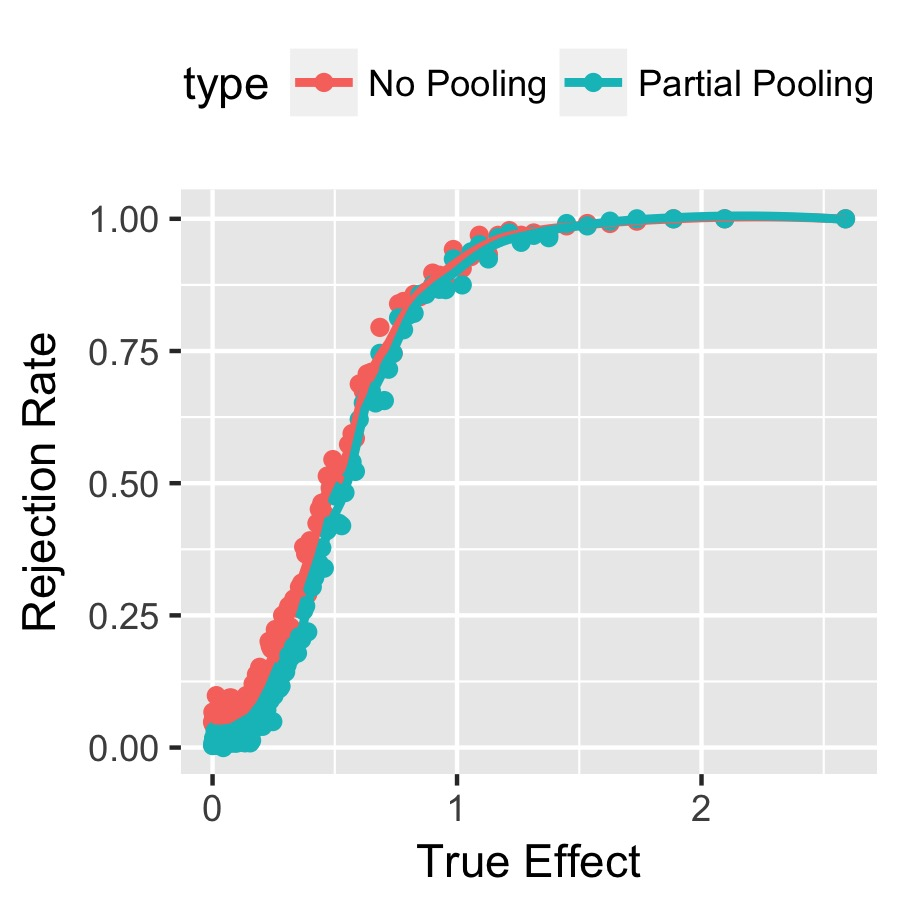
\includegraphics[width=0.5\textwidth]{reject.jpg}
\caption{Power curves: the probability of a significant result as a function of the true effect, for the two estimators.}
\label{fig:power}
\end{figure*}


\begin{table*}
\centering
\begin{tabular}{rrlllll}
&&\multicolumn{5}{c}{$\tau$}\\
&&0&0.1&0.2&0.5&1\\
\hline
\multirow{2}{*}{$Pr(\text{p-val}<0.05)$}& Partial Pooling & 0.00&0.01&0.03&0.31&0.61 \\ 
& No Pooling & 0.05&0.07&0.13&0.36&0.61 \\ 
\hline\multirow{2}{*}{$Pr(\text{At least one p-val}<0.05)$}& Partial Pooling & 0.02&0.08&0.33&1.00&1.00 \\ 
& No Pooling & 0.65&0.78&0.94&1.00&1.00 \\ 
\hline\multirow{2}{*}{ $Pr(\text{Wrong Sign}|\text{p-val}<0.05)$ }& Partial Pooling & 0.00&0.16&0.04&0.01&0.00 \\ 
& No Pooling & 0.00&0.18&0.06&0.01&0.00 \\ 
\hline\multirow{2}{*}{ $\EE\left[|\hat{d}/d||\text{p-val}<0.05\right]$ }& Partial Pooling &  &30.65&3.64&1.89&1.20 \\ 
& No Pooling &  &29.48&6.35&3.70&1.36 \\ 
\hline
\end{tabular}
\caption{The overall probability of a significant result, the probability of at least one significant result in a batch of 20 experiments, the proportion of significant results that were of the wrong sign, and the average ratio of the magnitudes of significant estimates to true effects for partial pooling and no pooling estimates for different values of $\tau$, the standard deviation of treatment effects, in the simulation study.}
\label{tab:simRes2}
\end{table*}

We present the simulation results in two parts. 
Table \ref{tab:simRes1} gives the results of the the simulation in terms of estimation. 
The estimated standard errors and root mean squared errors of partial pooling estimates were consistently substantially lower than those of no-pooling estimates.
In this context, partial pooling estimators were consistently more precise and accurate than their no-pooling counterparts. 
The differences between the estimators diminished as the variance of true treatment effects, $\tau$ increased. 
This is to be expected from (\ref{eq:shrinkageCoef}): as $\tau$ increases relative to no-pooling standard errors $\sigma$ (which in the simulation , the shrinkage coefficient tends towards 1 and the the partial pooling estimate tends towards the no-pooling estimate.
Intuitively, when $\tau$ increases various experiments become less informative about each other, so partial pooling decreases in value. 

Table \ref{tab:simRes1} also shows that while the no-pooling estimates are unbiased, the partial pooling estimates are slightly biased towards zero, as expected, with the bias decreasing as $\tau$ increases.

This bias does not cause undercoverage of 95\% confidence intervals.
In fact, for low $\tau$, the partial pooling confidence intervals \emph{over}-covered---more than 95\% of the realized confidence intervals included the true parameter. 
The width of the confidence interval is four times the standard error, by construction---so partial-pooling confidence intervals were substantially smaller than their no-pooling counterparts, without sacrificing coverage (and in some cases improving coverage). 

Table \ref{tab:simRes2} gives simulation results related to hypothesis testing. For every value of $\tau$, p-values from partial pooling estimators were less likely to be significant than those from no pooling estimators. 
Noting that even when $\tau$ is large some true effects are small, Figure \ref{fig:power} shows the probability of finding a significant effect as a function of the true effect for both estimators. 
For true effects less than 1, the partial pooling estimator is indeed more conservative. 

This conservativeness may be warranted---the last two lines of the table show that for low values of $\tau$ significant estimators (of both types) are often of the wrong size and/or too large. 
The second line of the table gives a result for multiplicity: the proportion of 20-experiment batches that contained a significant result. 
When $\tau=0$ and all effects were null, this is a type-I error rate under multiplicity.
The partial pooling estimator effectively controls multiplicity, with only two percent of batches containing a null result, while the no pooling estimator does not. 


\section{Discussion}

Partial pooling is a surprising, and surprisingly effective, technique to improve education sciences in the big data era. 
As educational technology allows A/B testing to proliferate, partial pooling is a method to use some of the oldest results in statistics---such as regression to the mean---alongside new Bayesian technology to improve precision and rein in false, un-replicable results. 
When experiments can be analyzed in a group, the result is smaller confidence intervals with the same or higher coverage, and fewer mistakes.

Partial pooling is a model based technique, and it remains to be shown that it performs well when the model is severely misspecified. 
What is the model's breaking point?
A host of Bayesian model checking procedures, including some suggested in \cite{rubin}, may be brought to bear on this question. 
In any event, most effect estimates are approximately normally distributed, by the central limit theorem, so methods based on normal theory will apply. 


\bibliographystyle{abbrv}
\bibliography{citations} 
\end{document}